\documentclass[12pt]{article}
\usepackage[T1]{fontenc}
\usepackage[utf8]{inputenc} 
\usepackage[a4paper]{geometry}
\usepackage{gensymb}
\geometry{a4paper, margin=1in}
\usepackage{natbib}
\usepackage{hyperref}
\usepackage{booktabs}
\usepackage{threeparttable}
\usepackage{amssymb}
\usepackage{amsmath}
\usepackage{graphicx}
\title{Assignment 5}
\author{Dmitrii Kuptsov}
\begin{document}
\maketitle
\section*{Task 1}

\subsection*{Task 1.a}

We estimate the following regression:

Model (1):
\begin{equation}
\ln(\text{medexp}) = \beta_1 + \beta_2 \text{privateins} + \beta_3 \text{phylum} + \beta_4 \text{actlim} + \beta_5 \text{totchr} + \beta_6 \text{age} + \beta_7 \text{female} + \varepsilon
\end{equation}

And get the following result:

\begin{figure}[h]
    \centering
    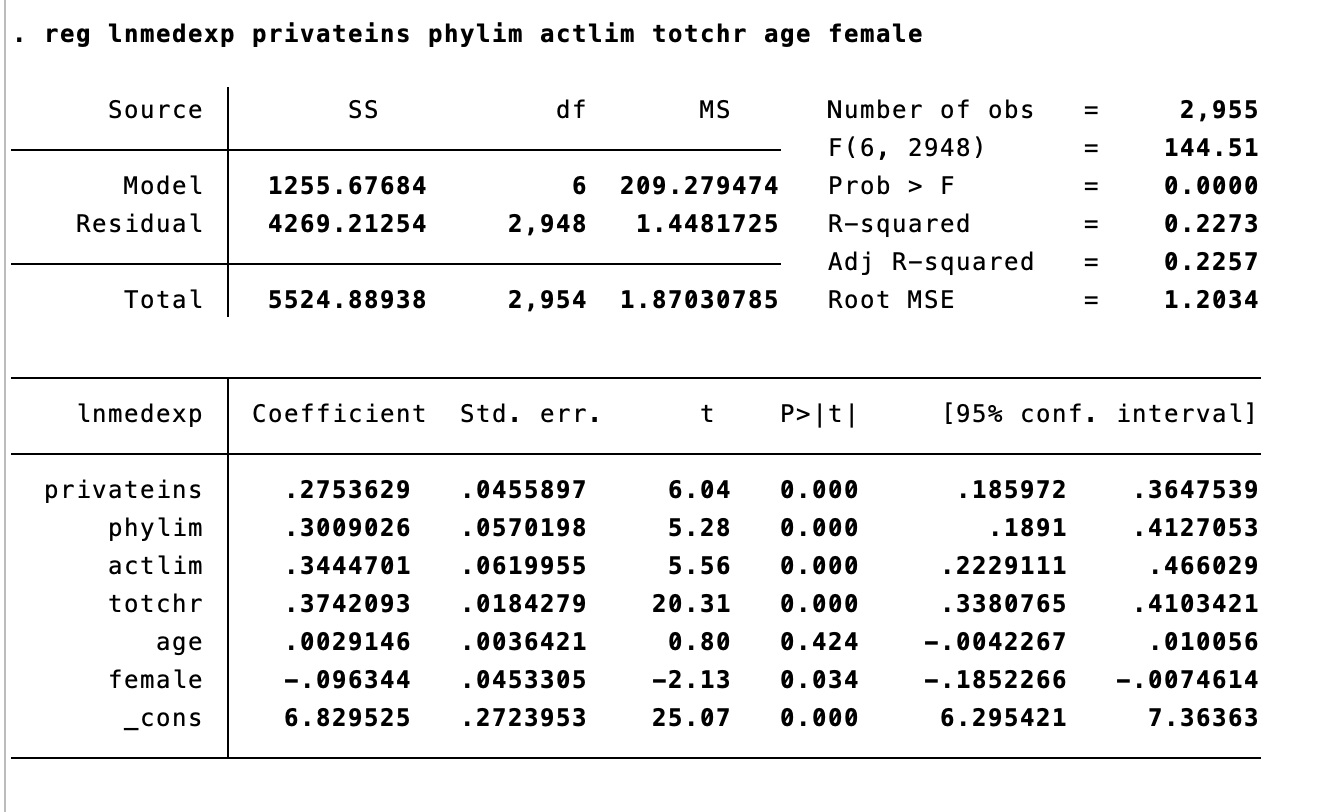
\includegraphics[width=\textwidth]{1_a.png}
    \caption{Results of the regression}
\end{figure}

\subsection*{Task 1.b}

$SE(\hat\beta_2) = \sqrt{\hat\sigma^2 \cdot (X^TX)^{-1}_{22}} = \sqrt{\frac{RSS}{N-K} \cdot (X^TX)^{-1}_{22}} = \sqrt{\frac{4269.}{2955 - 7} \cdot (X^TX)^{-1}_{22}} = \sqrt{1.448 \cdot (X^TX)^{-1}_{22}}$

\subsection*{Task 1.c}

$\beta_2$ captures the percentage difference in medical expenses between people who have private medical insurance and people who do not. The change in the outcome is measured in percentage points, because of the logarithm (let medexp = Y, privateins = X):

$d ln(Y)/dX = \frac{1}{Y}(\frac{dY}{dX}) = \beta_2 $
therefore
$ \frac{dY}{Y} = \beta_2 \cdot dX$

\subsection*{Task 1.d}

To check whether we are dealing with heteroskedastic disturbances, we would plot the fitted values of the outcome variable against the residuals. The homoskedasticity assumption states that disturbances have the same variance under different values of X. The predicted value of Y is the linear combination of X variables, so the errors should have approximately the same variance at different level of Y predicted under homoskedasticity.

Here is the plot:

\begin{figure}[h]
    \centering
    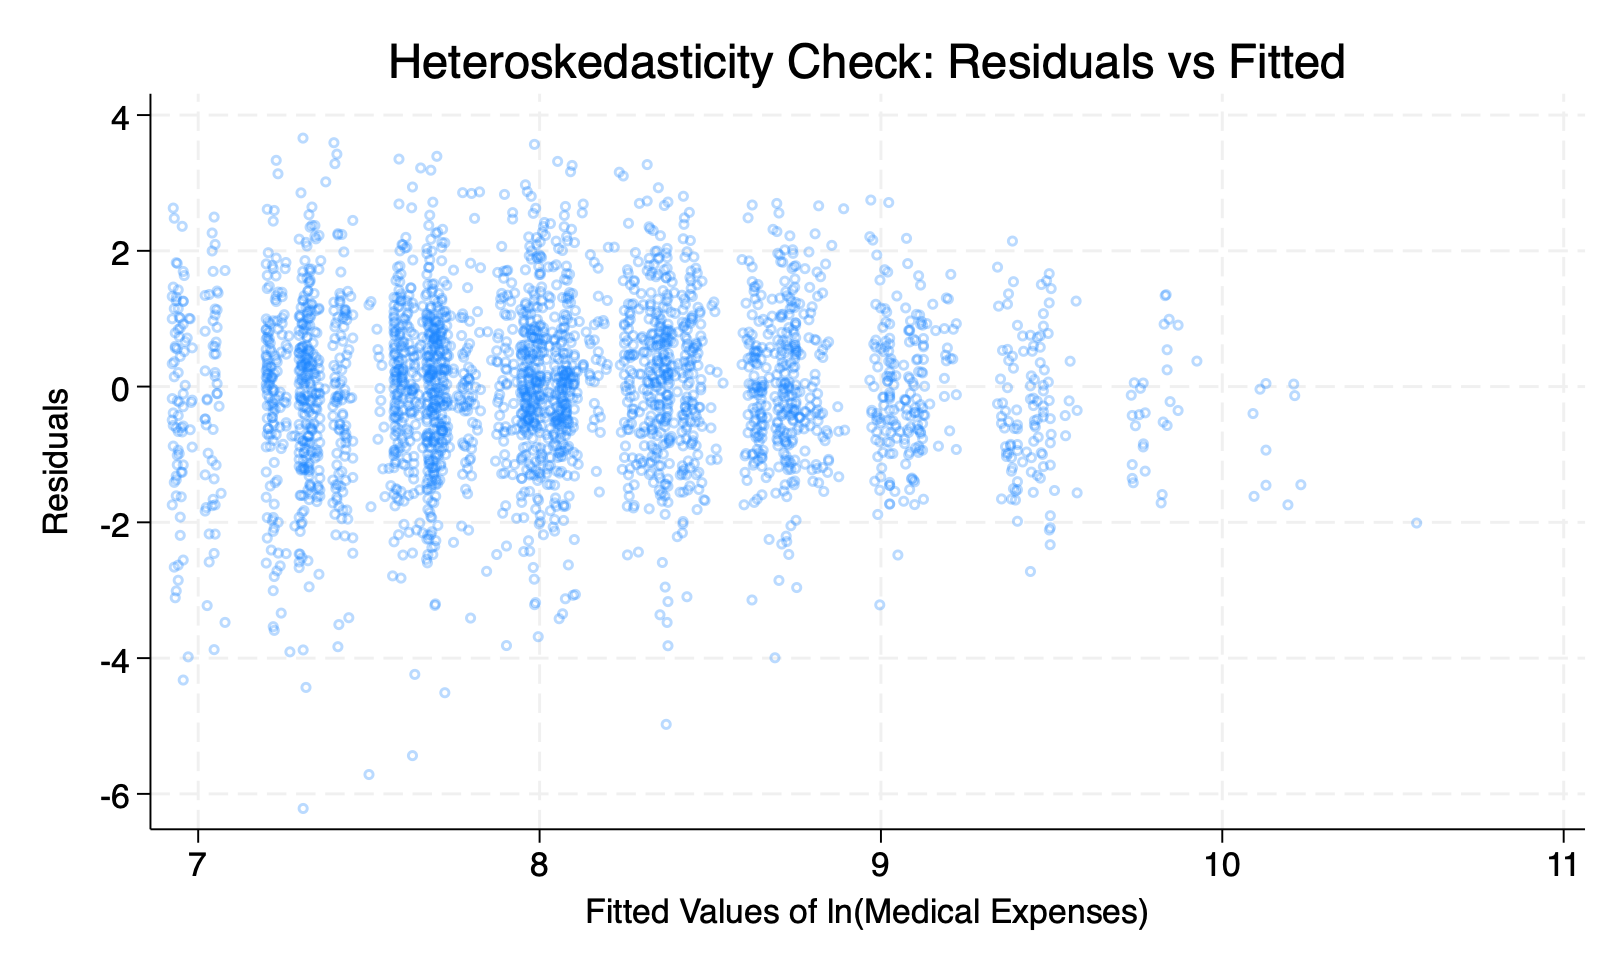
\includegraphics[width=\textwidth]{hetero_plot.png}
\end{figure}

It seems to us that some heteroskedacity is possible in this case, because for the higher level of the predicted outcome the variance of the errors seems lower than for the lower level of outcome. Therefore, there may be some unobservable factors that are correlated with the outcome. However, it should be further tested.

\subsection*{Task 1.e}

\subsubsection*{Task 1.e.i}

Here are the results we get from doing two steps from the assignment:

\begin{figure}[h]
    \centering
    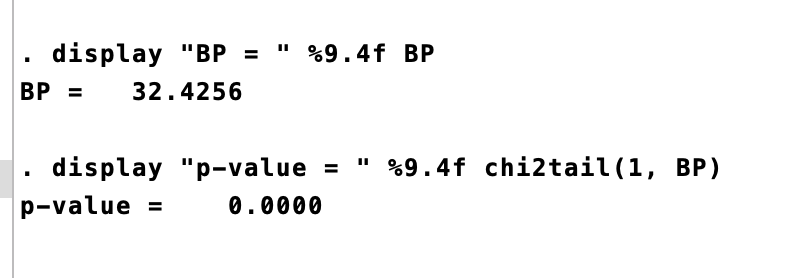
\includegraphics[width=0.7\textwidth]{1_e_i.png}
\end{figure}

It clearly shows the presence of heteroskedacity.

\subsubsection*{Task 1.e.ii}

Here are the results we get from "estat hettest , iid" command:

\begin{figure}[h]
    \centering
    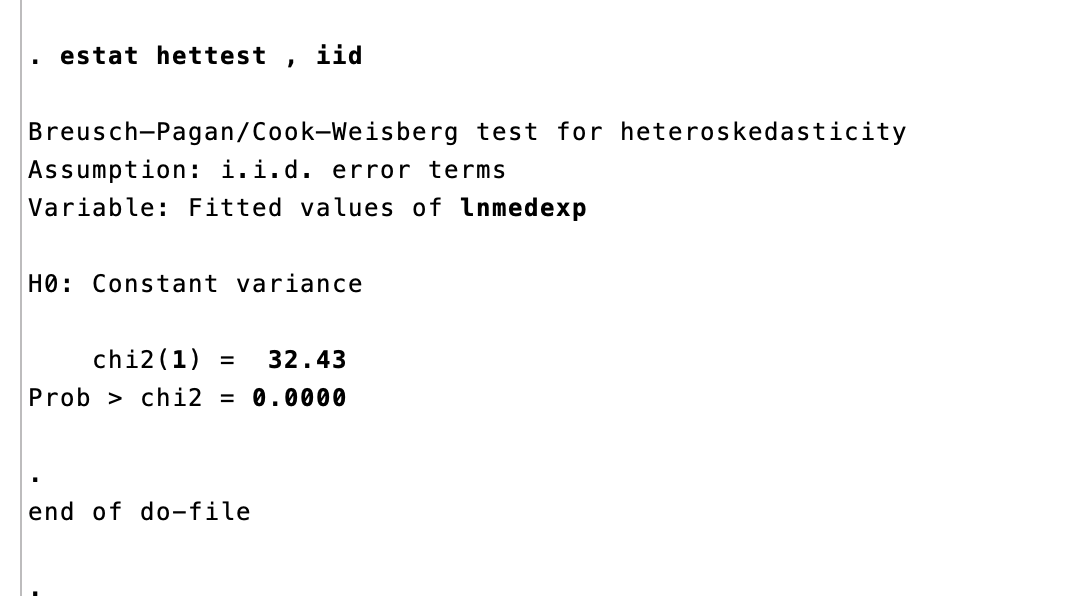
\includegraphics[width=0.7\textwidth]{1_e_ii.png}
\end{figure}

The BP statistic is the same as in the previous exercise.

\subsubsection*{Task 1.e.iii}

The output of the BP test was partly expected. We anticipated some level of heteroskedacity. However, the p-value seems very low, representing strong signs of heteroskedacity that we have not noticed.

\subsection*{Task 1.f}

It seems that we have to adjust the calculation of standard errors, because currently standard errors are computed under homoskedacity assumption that clearly does not hold in this case. So, the p-values and confidence intervals are incorrectly computed, therefore we have to compute heteroskedacity standard errors.

\subsection*{Task 1.g}

Here is the stata output with heteroskedacity-robust standard errors:

\begin{figure}[h]
    \centering
    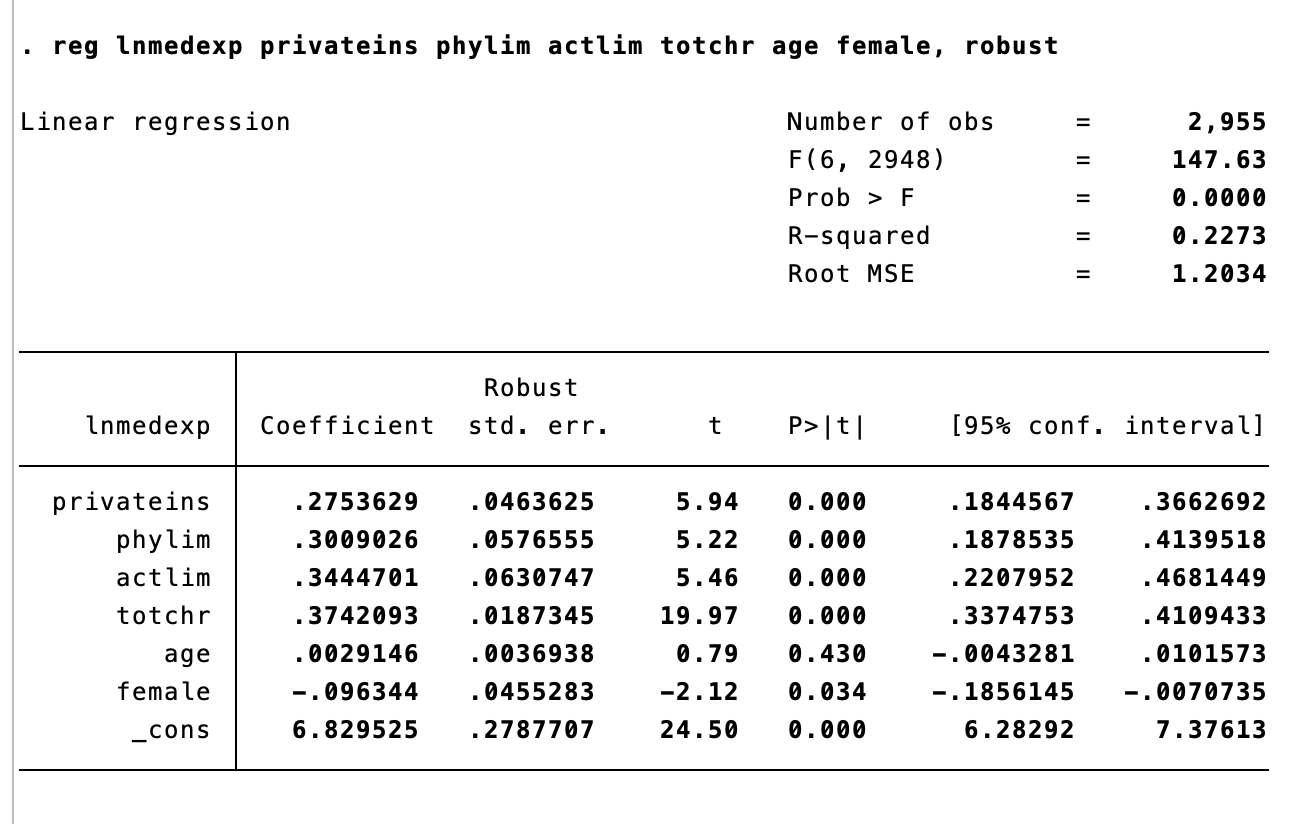
\includegraphics[width=\textwidth]{1_g.png}
\end{figure}

\subsection*{Task 1.h}

$R^2$ shouldn't change when moving from OLS estimation to robust OLS, because with this change the coefficients itself do not change. Therefore, fitted values and errors do not change, and so RSS and TSS do not change. Therefore, $R^2 = 1 - \frac{RSS}{TSS}$ does not change.

\subsection*{Task 1.i}


\end{document}
